%==============================================================================
%  Mini project report
%  Bayesian Networks and Markov Models in Action, 2026--2027
%
%  Every number, figure and table is produced by the code in ../code:
%  numbers and tables come from generated/ (code/make_report_numbers.py) and
%  figures from ../code/figures (code/fig_*.py), whose captions in the
%  appendices are written by the same scripts.
%==============================================================================
\documentclass[12pt]{article}

\usepackage[utf8]{inputenc}
\usepackage[T1]{fontenc}
\usepackage[english]{babel}
\usepackage{amsmath,amssymb,amsfonts}
\usepackage{graphicx}
\usepackage{booktabs}
\usepackage{xcolor}
\usepackage[ruled,vlined]{algorithm2e}
\usepackage[round]{natbib}
\usepackage[colorlinks=true,linkcolor=black,citecolor=blue,urlcolor=blue]{hyperref}

\usepackage{fancyhdr}
\pagestyle{fancy}

\usepackage[left=2.5cm,right=2.5cm,top=2.5cm,bottom=2.5cm]{geometry}
\setlength{\parskip}{6pt}

\usepackage[capitalise,noabbrev]{cleveref}

% Notation used in the course
\newcommand{\E}{\mathbb{E}}
\newcommand{\by}{\mathbf{y}}
\newcommand{\given}{\,\vert\,}
\newcommand{\logistic}{\operatorname{logit}^{-1}}
\newcommand{\Normal}{\mathcal{N}}
\newcommand{\Gam}{\text{Gamma}}
\newcommand{\sm}{\sigma_{\mathrm{m}}}
\newcommand{\sr}{\sigma_{\mathrm{r}}}
\newcommand{\spl}{\sigma_{\mathrm{p}}}
\newcommand{\taum}{\tau_{\mathrm{m}}}
\newcommand{\taur}{\tau_{\mathrm{r}}}
\newcommand{\taup}{\tau_{\mathrm{p}}}

\renewcommand{\headrulewidth}{0pt}
\pagestyle{fancy}
\fancyhead{}
\fancyfoot{}
\fancyfoot[L]{Bayesian Networks and Markov Models in Action}
\fancyfoot[R]{\thepage}

\graphicspath{{../code/figures/}}
% Written by code/make_report_numbers.py; do not edit.
\newcommand{\nRaw}{20{,}058}
\newcommand{\nDuplicates}{945}
\newcommand{\nShort}{576}
\newcommand{\nDraws}{855}
\newcommand{\nDecisive}{17{,}682}
\newcommand{\shareDraws}{4.6}
\newcommand{\shareWhiteDecisive}{52.1}
\newcommand{\nOpenings}{359}
\newcommand{\medianGamesOpening}{10}
\newcommand{\nOpeningsOne}{47}
\newcommand{\nPlayers}{14{,}832}
\newcommand{\shareRated}{81.4}
\newcommand{\shareFifteen}{7.3}
\newcommand{\nPairs}{203}
\newcommand{\nFirstMoves}{20}
\newcommand{\priorWinLow}{27}
\newcommand{\priorWinHigh}{73}
\newcommand{\priorSpreadLow}{0.13}
\newcommand{\priorSpreadHigh}{0.99}
\newcommand{\priorSpreadBelowTenth}{0.67}
\newcommand{\advantageEco}{23.5}
\newcommand{\advantageEcoLow}{13.9}
\newcommand{\advantageEcoHigh}{33.1}
\newcommand{\pShapeEco}{0.026}
\newcommand{\gridMaxZ}{1.04}
\newcommand{\isMaxZ}{1.96}
\newcommand{\pymcMaxZ}{1.26}
\newcommand{\pShapeOneAll}{0.027}
\newcommand{\pShapeOneRated}{0.006}
\newcommand{\pShapeOneUnrated}{<0.001}
\newcommand{\pShapeTwoAll}{0.331}
\newcommand{\betaRated}{1.76}
\newcommand{\betaRatedLow}{1.68}
\newcommand{\betaRatedHigh}{1.85}
\newcommand{\betaDiff}{0.54}
\newcommand{\betaDiffLow}{0.40}
\newcommand{\betaDiffHigh}{0.68}
\newcommand{\sigmaMove}{0.22}
\newcommand{\sigmaMoveLow}{0.13}
\newcommand{\sigmaMoveHigh}{0.34}
\newcommand{\sigmaReply}{0.13}
\newcommand{\sigmaReplyLow}{0.09}
\newcommand{\sigmaReplyHigh}{0.19}
\newcommand{\sigmaPlayer}{0.57}
\newcommand{\sigmaPlayerLow}{0.52}
\newcommand{\sigmaPlayerHigh}{0.63}
\newcommand{\sigmaPlayerPoints}{130}
\newcommand{\sigmaPlayerPointsLow}{117}
\newcommand{\sigmaPlayerPointsHigh}{144}
\newcommand{\advantageEfour}{24.5}
\newcommand{\advantageEfourLow}{4.8}
\newcommand{\advantageEfourHigh}{44.9}
\newcommand{\pWhiteEfour}{52.7}
\newcommand{\pWhiteEfourLow}{50.5}
\newcommand{\pWhiteEfourHigh}{54.9}
\newcommand{\pWhiteDfour}{52.1}
\newcommand{\pWhiteDfourLow}{49.4}
\newcommand{\pWhiteDfourHigh}{54.8}
\newcommand{\eloRatio}{0.77}
\newcommand{\eloRatioLow}{0.73}
\newcommand{\eloRatioHigh}{0.80}
\newcommand{\probAdvantageEfour}{0.979}
\newcommand{\probMoveMatters}{0.89}
\newcommand{\pWhiteEthree}{41.6}
\newcommand{\pWhiteEthreeLow}{35.3}
\newcommand{\pWhiteEthreeHigh}{47.6}
\newcommand{\pWhiteCfour}{54.2}
\newcommand{\pWhiteCfourLow}{50.1}
\newcommand{\pWhiteCfourHigh}{58.4}
\newcommand{\pWhiteSicilian}{50.7}
\newcommand{\pWhiteSicilianLow}{48.7}
\newcommand{\pWhiteSicilianHigh}{52.7}
\newcommand{\pWhiteOpenGame}{53.6}
\newcommand{\pWhiteOpenGameLow}{52.3}
\newcommand{\pWhiteOpenGameHigh}{54.9}
\newcommand{\probSicilian}{0.978}
\newcommand{\favouriteTwoHundred}{70.7}
\newcommand{\favouriteTwoHundredLow}{69.8}
\newcommand{\favouriteTwoHundredHigh}{71.5}
\newcommand{\eloTwoHundred}{76.0}
\newcommand{\rhatFinal}{1.007}
\newcommand{\essFinalShared}{1{,}114}
\newcommand{\essFinalFirstMoves}{852}
\newcommand{\essFinalPairs}{1{,}096}
\newcommand{\essFinalPlayers}{2{,}554}
\newcommand{\acceptPlayers}{0.44}
\newcommand{\acceptTheta}{0.36}
\newcommand{\dispersionWithout}{2.14}
\newcommand{\dispersionWithoutLow}{0.91}
\newcommand{\dispersionWithoutHigh}{1.10}
\newcommand{\pDispersionWithout}{<0.001}
\newcommand{\dispersionWith}{1.06}
\newcommand{\dispersionWithLow}{0.91}
\newcommand{\dispersionWithHigh}{1.10}
\newcommand{\pDispersionWith}{0.23}
\newcommand{\pChecksFinalLow}{0.12}
\newcommand{\pChecksFinalHigh}{0.81}
\newcommand{\biasSigmaReply}{0.049}
\newcommand{\biasSigmaReplySe}{0.002}
\newcommand{\biasSigmaMove}{0.040}
\newcommand{\biasSigmaMoveSe}{0.006}
\newcommand{\insideSigmaReply}{45}
\newcommand{\nRepeatsFull}{40}
\newcommand{\sensSicilianLow}{0.94}
\newcommand{\sensSicilianHigh}{0.98}
\newcommand{\sensEfourLow}{52.1}
\newcommand{\sensEfourHigh}{52.8}
\newcommand{\sensMoveLow}{0.77}
\newcommand{\sensMoveHigh}{0.91}
\newcommand{\sensEthreeLow}{0.986}
\newcommand{\sensPlayerBaseline}{0.57}
\newcommand{\sensPlayerRatedOnly}{0.44}
\newcommand{\sensPlayerNoFifteen}{0.47}
\newcommand{\sensRhatOthers}{1.010}
\newcommand{\sensRhatDiffuse}{1.020}
\newcommand{\nVariants}{9}


\begin{document}

%--------------------------------------------------------------------------
%  Title and authors
%--------------------------------------------------------------------------

\begin{center}
{\Large
	{\sc Who controls White's first-move advantage?\\[2pt] A hierarchical Bayesian model of online chess games}
}
\bigskip

\underline{Walid Ajbar} $^{1}$ \& Millan Das $^{2}$
\bigskip

{\it
$^{1}$ CentraleSup\'elec, France, walid.ajbar@student-cs.fr\\
$^{2}$ CentraleSup\'elec, France, millan.das@student-cs.fr
}
\end{center}

%--------------------------------------------------------------------------
%  Abstract
%--------------------------------------------------------------------------

{\bf Abstract.} White moves first and wins more often than Black, but how large this advantage is once ratings are accounted for, and how much each player's opening choice changes it, is uncertain. We model \nDecisive{} decisive Lichess games with a Bayesian logistic regression on the rating gap in which White's first move and Black's reply have hierarchical effects and each player has an effect for being stronger or weaker than their rating. We fit it with a Metropolis-within-Gibbs sampler that we implemented and validated on simulated games; the model was reached in steps, each answering a failure of the previous one. At equal ratings White wins \pWhiteEfour\% of decisive games after 1.e4 (90\% interval \pWhiteEfourLow{} to \pWhiteEfourHigh), worth \advantageEfour{} rating points, but Black's Sicilian reply leaves White only \pWhiteSicilian\%, against \pWhiteOpenGame\% after 1...e5 (posterior probability \probSicilian{} that it is the better reply). Ratings predict results less well than the Elo formula promises, and players of equal rating differ in strength by about \sigmaPlayerPoints{} points.

{\bf Keywords.} Bayesian inference; hierarchical model; Metropolis-within-Gibbs; posterior predictive checks; chess.

%--------------------------------------------------------------------------
\section{Introduction}\label{sec:introduction}
%--------------------------------------------------------------------------

In chess White moves first, and in almost every collection of games White wins more often than Black. How large is this first-move advantage once the players' strength is accounted for, and who controls it: White's first move, or Black's reply? The answer is uncertain because the advantage is small next to the effect of the rating gap, most opening lines are rarely played, and the same players appear in many games.

A Bayesian hierarchical model addresses all three: it estimates each opening effect with partial pooling, gives each conclusion as a posterior probability, and can carry an effect for each player. We built it in steps. A first model with one effect per opening code gave a robust first-move advantage, but it could tell few openings apart, its codes mix the moves of both players, and posterior predictive checks of it and of the next models found two features of the data they could not reproduce. Each later model answers one of these failures and was validated on simulated data before being fitted to the real games, with samplers we implemented following the course \citep{course2026notes}.

%--------------------------------------------------------------------------
\section{Data}\label{sec:data}
%--------------------------------------------------------------------------

We use the Chess Game Dataset of the Lichess server \citep{lichess2017kaggle}, public domain (CC0): \nRaw{} online games with the result, both players' identifiers and ratings at the time of the game, whether it was rated, and the moves. We removed \nDuplicates{} repeated game identifiers, \nShort{} games of fewer than 10 plies (abandoned rather than played) and \nDraws{} draws (\shareDraws\%; scoring them as half a win is a sensitivity check), leaving \nDecisive{} decisive games between \nPlayers{} players, \shareRated\% of them rated. For game $i$ we keep White's result $y_i$, the rating gap $\Delta_i$ (White minus Black, divided by 400, the Elo scale), the group $g(i)$ (rated or unrated), the opening code, and White's first move and Black's reply. White wins \shareWhiteDecisive\% of the decisive games; \cref{fig:data} shows the two features any model must capture.

\begin{figure}[t]
  \centering
  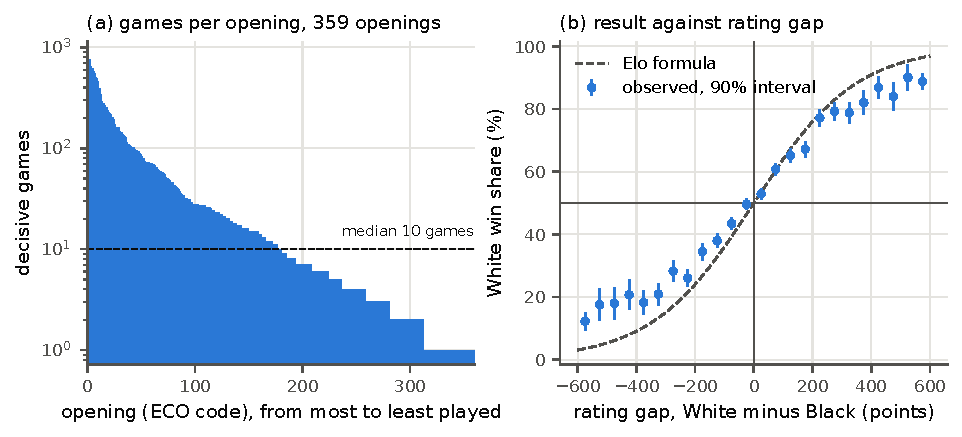
\includegraphics[width=0.86\linewidth]{data.pdf}
  \caption{(a) Decisive games per opening code, on a log scale: the median code has \medianGamesOpening{} games and \nOpeningsOne{} have one, so effects must be pooled across openings. (b) White's win share in 50-point bins of rating gap, with 90\% binomial intervals; the dashed line is the Elo expected score. The rating gap drives the result, with a flatter curve than Elo's, and White wins more than half of the games at equal rating.}
  \label{fig:data}
\end{figure}

%--------------------------------------------------------------------------
\section{Model}\label{sec:model}
%--------------------------------------------------------------------------

\paragraph{Why each part of the model.} We added a part only when the simpler model failed a check or could not answer the question. $M_0$ has $\Pr(y_i = 1) = \logistic(\theta_{o(i)} + \beta \Delta_i)$ with one effect $\theta_o \sim \Normal(\mu, \sigma^2)$ for each of the \nOpenings{} opening codes. Its posterior predictive check failed on the win share against the rating gap, so $M_1$ has one slope $\beta_g$ per group $g$. An opening code mixes the moves of both players and cannot say who controls the advantage, so $M_2$ uses the pair $c = (m, r)$ of White's first move $m$ and Black's reply $r$ in a two-level hierarchy. The games of a player were not independent given $M_2$, so the final model $M_3$ adds one effect per player.

\paragraph{Final model.} Game $i$ is played by White $w(i)$ against Black $b(i)$ in pair $c(i)$, whose first move is $m(c(i))$ (\cref{fig:model_full}):
\begin{gather}
  y_i \sim \text{Bernoulli}\big(\logistic(\eta_i)\big), \qquad \eta_i = \theta_{c(i)} + \beta_{g(i)} \Delta_i + u_{w(i)} - u_{b(i)}, \label{eq:likelihood}\\
  \theta_c \sim \Normal(\gamma_{m(c)}, \taur^{-1}), \qquad \gamma_m \sim \Normal(\mu, \taum^{-1}), \qquad u_p \sim \Normal(0, \taup^{-1}). \nonumber
\end{gather}
$\theta_c$ is White's advantage, on the log-odds scale, after the moves of pair $c$, for two players of equal rating and average strength for their rating; $\gamma_m$ is the advantage of first move $m$ averaged over replies and $\mu$ the average over the \nFirstMoves{} first moves; $\beta_g$ is the effect of the rating gap; and $u_p$ is how much stronger ($u_p > 0$) or weaker player $p$ is than their rating. We report the spreads $\sm = \taum^{-1/2}$ between first moves, $\sr = \taur^{-1/2}$ between replies to one first move and $\spl = \taup^{-1/2}$ between players. The unknowns are $\beta_1, \beta_2, \mu$, the three precisions, \nFirstMoves{} effects $\gamma_m$, \nPairs{} effects $\theta_c$ and \nPlayers{} effects $u_p$, and the posterior is, up to a constant,
\begin{equation}\label{eq:posterior}
\begin{split}
  \pi(\cdot \given \by) \propto{}& \prod_i \logistic(\eta_i)^{y_i} \big(1 - \logistic(\eta_i)\big)^{1 - y_i}
  \prod_c \Normal(\theta_c \given \gamma_{m(c)}, \taur^{-1})\\
  &\times \prod_m \Normal(\gamma_m \given \mu, \taum^{-1}) \prod_p \Normal(u_p \given 0, \taup^{-1})\;
  \pi(\mu)\, \pi(\beta_1)\, \pi(\beta_2)\, \pi(\taum)\, \pi(\taur)\, \pi(\taup).
\end{split}
\end{equation}

\begin{figure}[t]
  \centering
  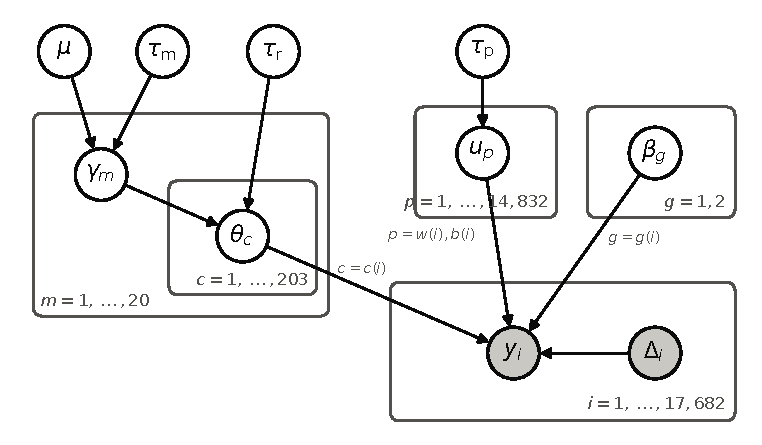
\includegraphics[width=0.66\linewidth]{model_full.pdf}
  \caption{The final model as a Bayesian network. Shaded nodes are observed, white nodes unknown; plates repeat their content for the \nFirstMoves{} first moves $m$, the \nPairs{} pairs $c$ of a first move and a reply (nested in their first move), the \nPlayers{} players $p$, the two groups $g$ (rated, unrated) and the \nDecisive{} games $i$. The likelihood and priors are \eqref{eq:likelihood} and \cref{sec:model}.}
  \label{fig:model_full}
\end{figure}

\paragraph{Priors.} The priors are independent. $\mu \sim \Normal(0, 0.5^2)$ puts 95\% of its mass on a win probability between 27\% and 73\% at equal ratings. $\beta_g \sim \Normal(\log 10, 1)$ is centred on the Elo formula \citep{elo1978rating}, whose expected score $1/(1 + 10^{-\text{gap}/400})$ equals $\logistic(\log(10)\Delta)$; its standard deviation of 1 leaves the slope to the data, since Lichess ratings are Glicko-2 ratings \citep{glickman2001dynamic}, not Elo. The precisions $\taum, \taur, \taup \sim \Gam(1, 0.05)$ (shape, rate) are conjugate to the Normal levels; this prior gives a spread between $0.13$ and $1$ with 90\% probability.

\paragraph{Assumptions.} Given the parameters the games are independent, the rating gap acts linearly on the log-odds within each group, and opening and player effects do not depend on the rating level. Players choose their openings, so the effects are associations given the ratings and player effects, not the effect of imposing a move.

%--------------------------------------------------------------------------
\section{Method}\label{sec:method}
%--------------------------------------------------------------------------

We sample \eqref{eq:posterior} with the Metropolis-within-Gibbs sampler of \cref{alg:sampler}, written in Python with NumPy \citep{harris2020array}; \cref{app:conditionals} derives the full conditionals. $\theta_c$, $\beta_g$ and $u_p$ have no standard full conditional and get random-walk Metropolis--Hastings steps. Given the rest, the pairs are independent, as are the two slopes, so each block moves in one vectorized sweep with an accept step per component. Two players who meet share a game, so we colour the graph whose edges are the games: players of one colour never meet, are independent given the rest, and move together; a greedy colouring needs only 4 colours. $\gamma_m$, $\mu$ and the precisions have conjugate Normal and Gamma full conditionals.

\begin{algorithm}[t]
\caption{One iteration of the sampler of the final model.}\label{alg:sampler}
\DontPrintSemicolon
update every $\theta_c$ by random-walk Metropolis--Hastings, in one vectorized sweep\;
rescale the replies: $\theta_c' = \gamma_{m(c)} + e^{\varepsilon}(\theta_c - \gamma_{m(c)})$, $\taur' = e^{-2\varepsilon}\taur$, $\varepsilon \sim \Normal(0, s_{\mathrm{r}}^2)$; accept or reject\;
update $\beta_1, \beta_2$ by random-walk Metropolis--Hastings\;
\For{each colour of players}{update all its $u_p$ by random-walk Metropolis--Hastings, each with its own accept step\;}
rescale the players: $u' = e^{\varepsilon} u$, $\taup' = e^{-2\varepsilon}\taup$, $\varepsilon \sim \Normal(0, s_{\mathrm{p}}^2)$; accept or reject\;
draw each $\gamma_m$, then $\mu$, from their Normal full conditionals, and $\taur, \taum, \taup$ from their Gamma full conditionals\;
\end{algorithm}

\paragraph{Rescaling moves.} Most players have one or two games, so each $u_p$ is held near the current spread and the spread near the $u_p$: one-at-a-time updates creep along this funnel, and in a first version the player spread had an effective sample size of 6 from 20{,}000 draws on simulated data. The rescaling moves of \cref{alg:sampler} move a level and its precision together \citep{liu2000generalised}. They leave the Normal prior of the level invariant, so the acceptance probability is $\min\{1, \exp(\Delta\ell - 2a\varepsilon - b\tau(e^{-2\varepsilon} - 1))\}$ with $\Delta\ell$ the change of log-likelihood and $(a, b) = (1, 0.05)$ (\cref{app:conditionals}); the same quantity then reached an effective sample size of 399.

\paragraph{Tuning and runs.} Each proposal scale is 2.38 posterior standard deviations \citep{roberts1997weak}, estimated on the second half of a 3{,}000-iteration pilot run; median acceptance rates are then \acceptTheta{} for the pairs and \acceptPlayers{} for the players. We run 4 chains from points drawn from the prior, discard 2{,}000 iterations and keep 40{,}000 per chain (12 minutes with parallel chains), and check them with split-$\hat R$ \citep{gelman1992inference} and effective sample sizes from Geyer's initial positive sequence \citep{geyer1992practical}, which we implemented.

%--------------------------------------------------------------------------
\section{Validation on simulated data}\label{sec:validation}
%--------------------------------------------------------------------------

Each model was validated before its first real fit, on games simulated from the model with the real rating gaps, groups, openings and players (\cref{tab:validation}). The decisive test draws the parameters of 100 data sets from the prior: if the sampler is correct, the posterior intervals then contain the truth at their nominal rate, whatever the prior. They do, for every parameter of every model, including the \nPlayers{} player effects (\cref{fig:validation_full} in \cref{app:figures}). For $M_0$ Metropolis--Hastings also matches, within \gridMaxZ, \isMaxZ{} and \pymcMaxZ{} Monte Carlo standard errors, an exact grid integration on a small problem, importance sampling with a Laplace proposal without openings, and PyMC \citep{abrilpla2023pymc}, used only as a cross-check.

\begin{table}[t]
  \centering
  \caption{Validation on simulated games. Second column: shared parameters whose true value lies in its 90\% posterior interval, for one data set simulated with chosen values. Coverage: lowest to highest share, over all parameters and effects, of the posterior intervals that contain the true value, over 100 data sets whose parameters are drawn from the prior.}
  \label{tab:validation}
  \small
  % Written by code/make_report_numbers.py; do not edit.
\begin{tabular}{@{}lccc@{}}
\toprule
Model & True values inside & \multicolumn{2}{c}{Coverage over 100 data sets} \\
 & 90\% intervals (one data set) & 50\% intervals & 90\% intervals \\
\midrule
First model (ECO openings) & 2 of 3 & 46--58\% & 90--94\% \\
+ rated and unrated slopes & 4 of 4 & 45--52\% & 86--93\% \\
First move and reply & 5 of 5 & 48--56\% & 87--90\% \\
Final model (+ player effects) & 3 of 6 & 48--54\% & 84--94\% \\
\bottomrule
\end{tabular}

\end{table}

With fixed chosen values, three of six true values of the final model fall outside their intervals. Refitting \nRepeatsFull{} data sets simulated with the same values separates chance from bias. The slopes, $\mu$ and $\spl$ show no bias, so their misses are chance; $\mu$ is the mean of only \nFirstMoves{} effects and the posterior targets their realized mean. The spread between replies is biased: $\sr$ is overestimated by \biasSigmaReply{} on average (standard error \biasSigmaReplySe) and contains its true value only \insideSigmaReply\% of the time, and $\sm$ is overestimated by \biasSigmaMove. The $\Gam(1, 0.05)$ prior puts less than 1\% of its mass on a spread as small as the chosen 0.10, and with few games per pair the data do not override it: the reported spreads between openings lean high.

%--------------------------------------------------------------------------
\section{Results}\label{sec:results}
%--------------------------------------------------------------------------

\paragraph{Diagnostics.} On the real games the four chains of the final model agree (trace plots in \cref{fig:trace_full}): the largest split-$\hat R$ over the shared parameters, first moves, pairs and players with at least 10 games is \rhatFinal, and the smallest effective sample sizes are \essFinalShared{} for the shared parameters ($\sm$, learned from \nFirstMoves{} first moves), \essFinalPairs{} for the pairs and \essFinalPlayers{} for the players, so Monte Carlo errors are small next to the posterior standard deviations.

\paragraph{One rating slope was not enough.} $M_0$ gives White an advantage of \advantageEco{} rating points (\advantageEcoLow{} to \advantageEcoHigh) and reproduces the overall win share and the spread between openings, but not the shape of the win share against the rating gap ($p = \pShapeEco$; \pShapeOneAll{} with a second set of replicates in \cref{fig:rating_slopes}). With one slope for rated and one for unrated games the check passes ($p = \pShapeTwoAll$, against \pShapeOneRated{} and \pShapeOneUnrated{} within each group with one slope; \cref{fig:rating_slopes}). In the final model the rated slope is \betaRated{} (\betaRatedLow{} to \betaRatedHigh), larger than the unrated one by \betaDiff{} (\betaDiffLow{} to \betaDiffHigh), and only \eloRatio{} of the Elo slope: after 1.e4 in rated games, a player of average strength rated 200 points higher wins \favouriteTwoHundred\% of decisive games, averaged over both colours (\favouriteTwoHundredLow{} to \favouriteTwoHundredHigh), not the \eloTwoHundred\% of the Elo formula.

\begin{figure}[t]
  \centering
  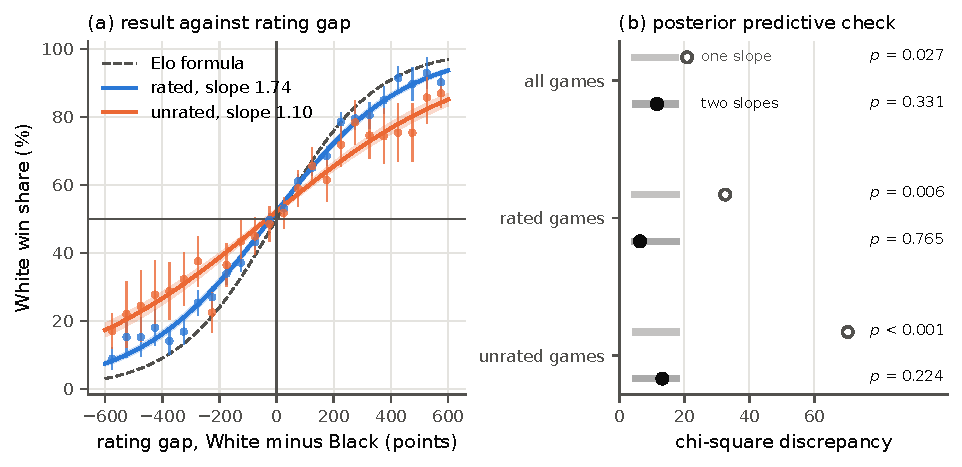
\includegraphics[width=0.86\linewidth]{rating_slopes.pdf}
  \caption{(a) White's win share by rating gap in rated and unrated games (50-point bins, 90\% binomial intervals), with the posterior mean and 90\% band of $\logistic(\mu + \beta_g \Delta)$ for the average opening of $M_1$ and the Elo expected score (dashed). (b) Posterior predictive check of the win share over deciles of the rating gap, as a chi-square discrepancy: realized value (dot), 90\% interval of its replicates (bar) and $p$-value, with one slope (open) and two (filled).}
  \label{fig:rating_slopes}
\end{figure}

\paragraph{Players needed their own effect.} For players with at least 10 games, the variance of the standardized difference between their score and the score expected without player effects is \dispersionWithout, while the model's replicates give \dispersionWithoutLow{} to \dispersionWithoutHigh{} ($p \pDispersionWithout$, \cref{fig:posterior_predictive_full}): the same players keep beating, or missing, their rating. With player effects it is \dispersionWith{} ($p = \pDispersionWith$) and every other check passes ($p$ from \pChecksFinalLow{} to \pChecksFinalHigh). Players of equal rating differ by $\spl = \sigmaPlayer$ (\sigmaPlayerLow{} to \sigmaPlayerHigh), or \sigmaPlayerPoints{} rating points.

\begin{figure}[t]
  \centering
  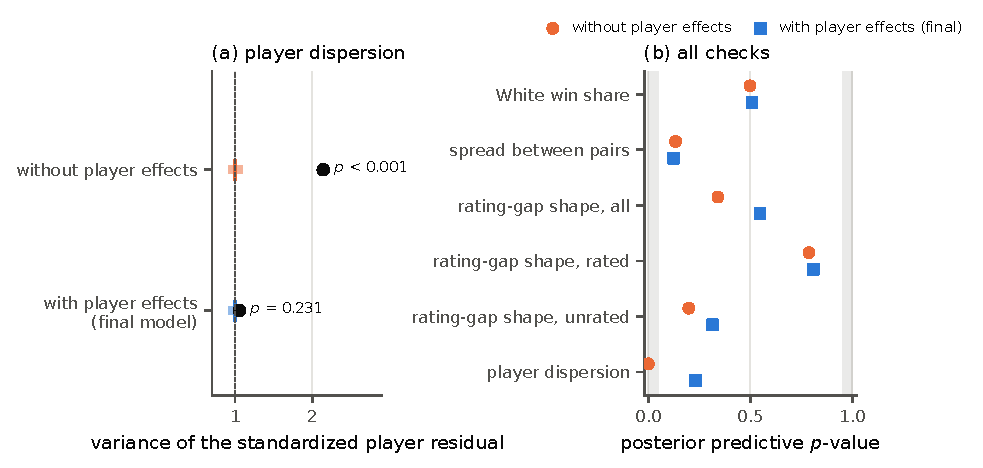
\includegraphics[width=0.86\linewidth]{posterior_predictive_full.pdf}
  \caption{Posterior predictive checks of the final model (blue) and of the same model without player effects (orange), from 4{,}000 simulated data sets each. (a) Variance of the standardized difference between score and expected score over players with at least 10 games: realized value (dot), 90\% interval and median of its replicates. (b) $p$-values of all checks; gray bands mark $p < 0.05$ or $p > 0.95$.}
  \label{fig:posterior_predictive_full}
\end{figure}

\paragraph{White's first move and Black's reply.} At equal ratings White wins \pWhiteEfour\% of decisive games after 1.e4 (\pWhiteEfourLow{} to \pWhiteEfourHigh), \advantageEfour{} rating points with probability \probAdvantageEfour{} of being positive, and \pWhiteDfour\% after 1.d4 (\cref{fig:moves}; all summaries in \cref{tab:final}). White's first move matters: after 1.e3 White wins only \pWhiteEthree\% (\pWhiteEthreeLow{} to \pWhiteEthreeHigh), while 1.c4 gives the most, \pWhiteCfour\%. Black's reply matters too: against 1.e4 the Sicilian, 1...c5, leaves White \pWhiteSicilian\% (\pWhiteSicilianLow{} to \pWhiteSicilianHigh), an interval containing 50\%, against \pWhiteOpenGame\% after 1...e5, with posterior probability \probSicilian{} that the Sicilian is the better reply for Black. The first move matters more than the reply, $\sm = \sigmaMove$ (\sigmaMoveLow{} to \sigmaMoveHigh) against $\sr = \sigmaReply$ (\sigmaReplyLow{} to \sigmaReplyHigh), with probability \probMoveMatters.

\begin{figure}[t]
  \centering
  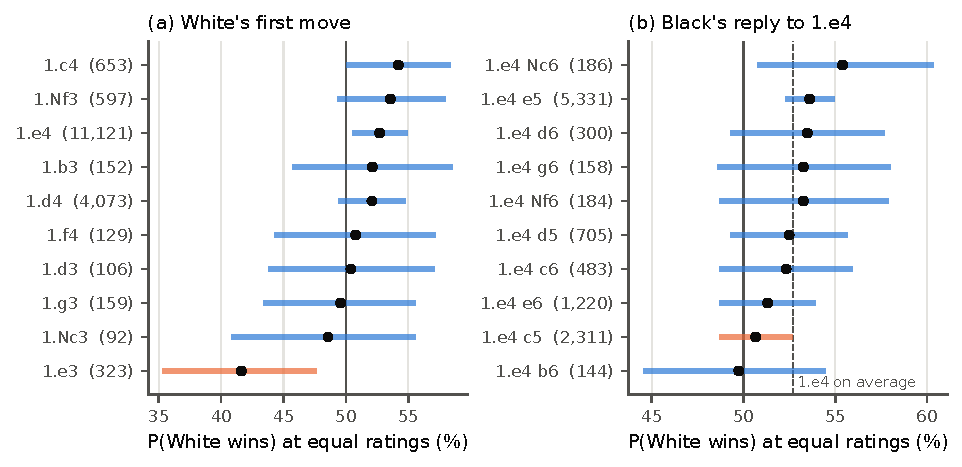
\includegraphics[width=0.86\linewidth]{moves.pdf}
  \caption{$\Pr(\text{White wins})$ at equal ratings in the final model, by White's first move (first moves with at least 90 games) and by Black's reply to 1.e4 (replies with at least 140 games): posterior means and 90\% intervals, number of decisive games in parentheses. The dashed line in (b) is 1.e4 on average; orange marks 1.e3 and the Sicilian.}
  \label{fig:moves}
\end{figure}

\paragraph{Sensitivity.} Across \nVariants{} variants of the priors and data (\cref{tab:sensitivity}), White wins \sensEfourLow\% to \sensEfourHigh\% after 1.e4, the Sicilian is the better reply with probability \sensSicilianLow{} to \sensSicilianHigh, and 1.e3 is worse than 1.e4 with probability at least \sensEthreeLow. The claim that the first move matters more than the reply is the most fragile (\sensMoveLow{} to \sensMoveHigh). The player spread is the most sensitive quantity: it falls from \sensPlayerBaseline{} to \sensPlayerRatedOnly{} on rated games only and to \sensPlayerNoFifteen{} without the players at the possible default rating of 1500 (\shareFifteen\% of games), so part of it comes from casual games and provisional ratings. All variants converge (split-$\hat R \le \sensRhatOthers$) except the diffuse prior, under which $\sm$ nears zero and the first-move level, without a rescaling move, mixes slowly ($\hat R = \sensRhatDiffuse$ with chains four times longer): its row agrees with the others but is indicative only.

\begin{table}[!ht]
  \centering
  \caption{Sensitivity of the final model to the priors (the three precisions share the prior on $\tau$) and to the games used: rated slope, player spread, $\Pr(\text{White wins})$ (\%) at equal ratings after 1.e4, 1.e4 c5 and 1.e4 e5, and the probability that the Sicilian is the better reply.}
  \label{tab:sensitivity}
  \small
  % Written by code/make_report_numbers.py; do not edit.
\begin{tabular}{@{}lrrrrrr@{}}
\toprule
Variant & Games & $\beta_{\mathrm{rated}}$ & $\sigma_{\mathrm{p}}$ & 1.e4, \% & 1.e4 c5 / e5, \% & $\Pr$(c5 better) \\
\midrule
baseline & 17{,}682 & 1.76 & 0.57 & 52.7 & 50.7 / 53.6 & 0.978 \\
tau Gamma(2, 0.1) & 17{,}682 & 1.76 & 0.57 & 52.8 & 50.6 / 53.6 & 0.980 \\
tau Gamma(0.5, 0.005) & 17{,}682 & 1.77 & 0.58 & 52.4 & 51.1 / 53.4 & 0.960 \\
mu sd 1 & 17{,}682 & 1.76 & 0.57 & 52.7 & 50.7 / 53.6 & 0.978 \\
beta N(0, 1) & 17{,}682 & 1.76 & 0.57 & 52.7 & 50.7 / 53.6 & 0.979 \\
rated games only & 14{,}397 & 1.75 & 0.44 & 52.5 & 50.6 / 53.5 & 0.973 \\
no player rated 1500 & 16{,}394 & 1.82 & 0.47 & 52.3 & 51.0 / 53.2 & 0.942 \\
draws as half wins & 18{,}537 & 1.67 & 0.44 & 52.5 & 50.6 / 53.3 & 0.980 \\
at least 20 plies & 16{,}741 & 1.75 & 0.55 & 52.1 & 50.7 / 53.0 & 0.939 \\
\bottomrule
\end{tabular}

\end{table}

%--------------------------------------------------------------------------
\section{Discussion and conclusion}\label{sec:discussion}
%--------------------------------------------------------------------------

White's first move is worth about \advantageEfour{} rating points after 1.e4 (\advantageEfourLow{} to \advantageEfourHigh), a win probability of \pWhiteEfour\% at equal ratings, but White can lose it with a weak first move such as 1.e3, and Black can almost cancel it with the Sicilian, under every prior and data variant we tried. Ratings also promise more than they deliver, and players of equal rating differ by about \sigmaPlayerPoints{} rating points.

\paragraph{Limitations.} The effects are associations: a player who chooses the Sicilian may differ from one who does not in ways that neither the rating nor the player effect captures. We noticed the Sicilian contrast while exploring the data, so its probability should be read with care, although hierarchical shrinkage guards against selecting chance extremes \citep{gelman2012multiple} and chess practice counts the Sicilian among Black's strongest replies to 1.e4. The games are amateur online games from a selection of users, the prior on the precisions pulls small spreads up, and draws are left out: next we would model draws as a third outcome, let player strength change over time, and use more games to estimate rare replies precisely.

%--------------------------------------------------------------------------
%  References (not counted in the 8 pages)
%--------------------------------------------------------------------------

\bibliographystyle{apalike}
\bibliography{references}

%--------------------------------------------------------------------------
%  Appendices (not counted in the 8 pages)
%--------------------------------------------------------------------------
\appendix
\crefalias{section}{appendix}

\section{Full conditional distributions}\label{app:conditionals}

Write $n_m$ for the number of pairs of first move $m$; $C$, $M$ and $P$ for the numbers of pairs, first moves and players; $(a, b)$ for the shape and rate of the Gamma priors; and $\mu_0, s_0$ for the mean and standard deviation of the prior of $\mu$. Each Normal level is conjugate to the level above it, and each Gamma prior to the Normal level it governs:
\begin{align*}
  \gamma_m \given \cdot &\sim \Normal\!\left(\frac{\taum \mu + \taur \sum_{c: m(c) = m} \theta_c}{\taum + n_m \taur}, \frac{1}{\taum + n_m \taur}\right),\\
  \mu \given \cdot &\sim \Normal\!\left(\frac{\mu_0 / s_0^2 + \taum \sum_m \gamma_m}{1/s_0^2 + M \taum}, \frac{1}{1/s_0^2 + M \taum}\right),\\
  \taur \given \cdot &\sim \Gam\Big(a + \tfrac{C}{2},\, b + \tfrac12 \sum_c (\theta_c - \gamma_{m(c)})^2\Big),\\
  \taum \given \cdot &\sim \Gam\Big(a + \tfrac{M}{2},\, b + \tfrac12 \sum_m (\gamma_m - \mu)^2\Big),\\
  \taup \given \cdot &\sim \Gam\Big(a + \tfrac{P}{2},\, b + \tfrac12 \sum_p u_p^2\Big).
\end{align*} Each follows from multiplying a Normal or Gamma density by Normal densities and completing the square, or collecting the powers of $\tau$. The full conditionals of $\theta_c$, $\beta_g$ and $u_p$ contain the logistic likelihood \eqref{eq:likelihood} and have no standard form; for example
\[
  \pi(\theta_c \given \cdot) \propto \prod_{i: c(i) = c} \logistic(\eta_i)^{y_i}\big(1 - \logistic(\eta_i)\big)^{1 - y_i}\; \exp\!\big\{-\tfrac{\taur}{2}(\theta_c - \gamma_{m(c)})^2\big\},
\]
hence their Metropolis--Hastings steps. The player effects $u_p$ of one colour share no game, so their full conditional factorizes over the players, and an accept step per player is valid.

\paragraph{Rescaling move.} The move maps $(\theta, \taur)$ to $(\theta', \taur')$ with $\theta_c' - \gamma_{m(c)} = e^{\varepsilon}(\theta_c - \gamma_{m(c)})$ and $\taur' = e^{-2\varepsilon}\taur$, for $\varepsilon$ drawn from a symmetric distribution; the move with $-\varepsilon$ undoes it, and its Jacobian is $e^{C\varepsilon}e^{-2\varepsilon}$. The Normal densities of the level satisfy $\prod_c \Normal(\theta_c' \given \gamma_{m(c)}, 1/\taur') = e^{-C\varepsilon}\prod_c \Normal(\theta_c \given \gamma_{m(c)}, 1/\taur)$, which cancels the factor $e^{C\varepsilon}$ of the Jacobian, and the Gamma prior contributes $(\taur'/\taur)^{a-1} e^{-b(\taur' - \taur)}$. The acceptance probability is therefore $\min\{1, \exp(\Delta\ell - 2a\varepsilon - b\taur(e^{-2\varepsilon} - 1))\}$, where $\Delta\ell$ is the change of the log-likelihood. The move for the players is the same with $u$, $\taup$ and $P$.

\section{Additional tables and figures}\label{app:figures}

\begin{table}[h]
  \centering
  \caption{Posterior means and 90\% intervals of the final model. Win probabilities are for two players of equal rating and average strength for their rating.}
  \label{tab:final}
  \small
  % Written by code/make_report_numbers.py; do not edit.
\begin{tabular}{@{}lrr@{}}
\toprule
Quantity & Mean & 90\% interval \\
\midrule
Slope $\beta_g$, rated games & 1.76 & 1.68 to 1.85 \\
Slope $\beta_g$, unrated games & 1.22 & 1.11 to 1.34 \\
Spread between first moves, $\sigma_{\mathrm{m}}$ & 0.22 & 0.13 to 0.34 \\
Spread between replies, $\sigma_{\mathrm{r}}$ & 0.13 & 0.09 to 0.19 \\
Spread between players, $\sigma_{\mathrm{p}}$ & 0.57 & 0.52 to 0.63 \\
\quad in rating points, $400\,\sigma_{\mathrm{p}}/\beta_{\mathrm{rated}}$ & 130 & 117 to 144 \\
White's edge after 1.e4, rating points & 24.5 & 4.8 to 44.9 \\
\midrule
\multicolumn{3}{@{}l}{$\Pr(\text{White wins})$ at equal ratings, \%} \\
\quad after 1.e4 & 52.7 & 50.5 to 54.9 \\
\quad after 1.d4 & 52.1 & 49.4 to 54.8 \\
\quad after 1.c4 & 54.2 & 50.1 to 58.4 \\
\quad after 1.e3 & 41.6 & 35.3 to 47.6 \\
\quad after 1.e4 e5 & 53.6 & 52.3 to 54.9 \\
\quad after 1.e4 c5 (Sicilian) & 50.7 & 48.7 to 52.7 \\
\quad after 1.e4 e6 (French) & 51.3 & 48.7 to 53.9 \\
\bottomrule
\end{tabular}

\end{table}

\Cref{tab:final} gives the posterior summaries of the final model, \cref{fig:validation_full} its validation on simulated games and \cref{fig:trace_full} its convergence on the real data.

\begin{figure}[htbp]
  \centering
  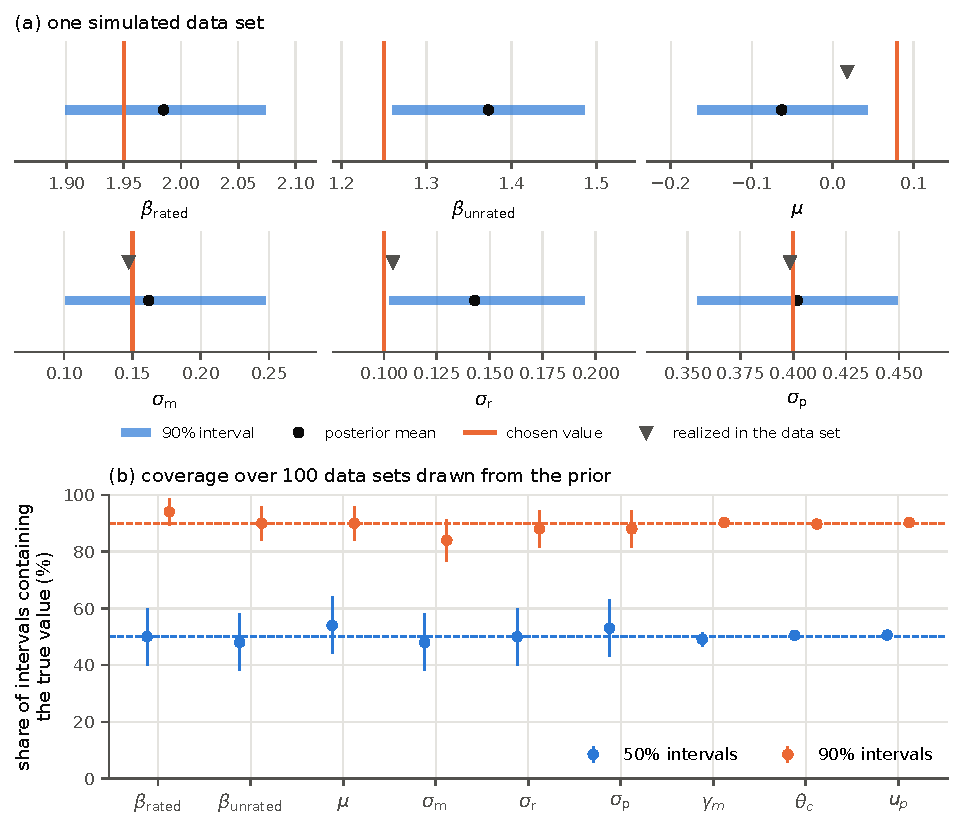
\includegraphics[width=\linewidth]{validation_full.pdf}
  \caption{Validation of the final model on simulated games, with the real rating gaps, rated status, pairs and players and the results drawn from the model. (a): one data set simulated with chosen values (orange lines); the posterior mean (black) and central 90\% interval (blue). The spreads and $\mu$ describe effects drawn once per data set, so the gray triangles mark the values realized in this data set, which the posterior targets. Over 40 data sets simulated with the same values, the slopes, $\mu$ and $\sigma_{\mathrm{p}}$ show no bias, but $\sigma_{\mathrm{r}}$ is overestimated by 0.049 on average (standard error 0.002) and $\sigma_{\mathrm{m}}$ by 0.040 (0.006): the $\text{Gamma}(1, 0.05)$ prior on the precisions puts less than 1\% of its mass on a spread as small as 0.10, and with few games per pair the data do not fully override it. (b): share of the 50\% and 90\% intervals that contain the true value, with $\pm 2$ standard errors, over 100 data sets whose parameters are drawn from the prior; for $\gamma_m$, $\theta_c$ and $u_p$ the share is over all first moves, pairs or players of all data sets. The shares match the nominal levels, as they must when the sampler is correct, whatever the prior.}
  \label{fig:validation_full}
\end{figure}

\begin{figure}[htbp]
  \centering
  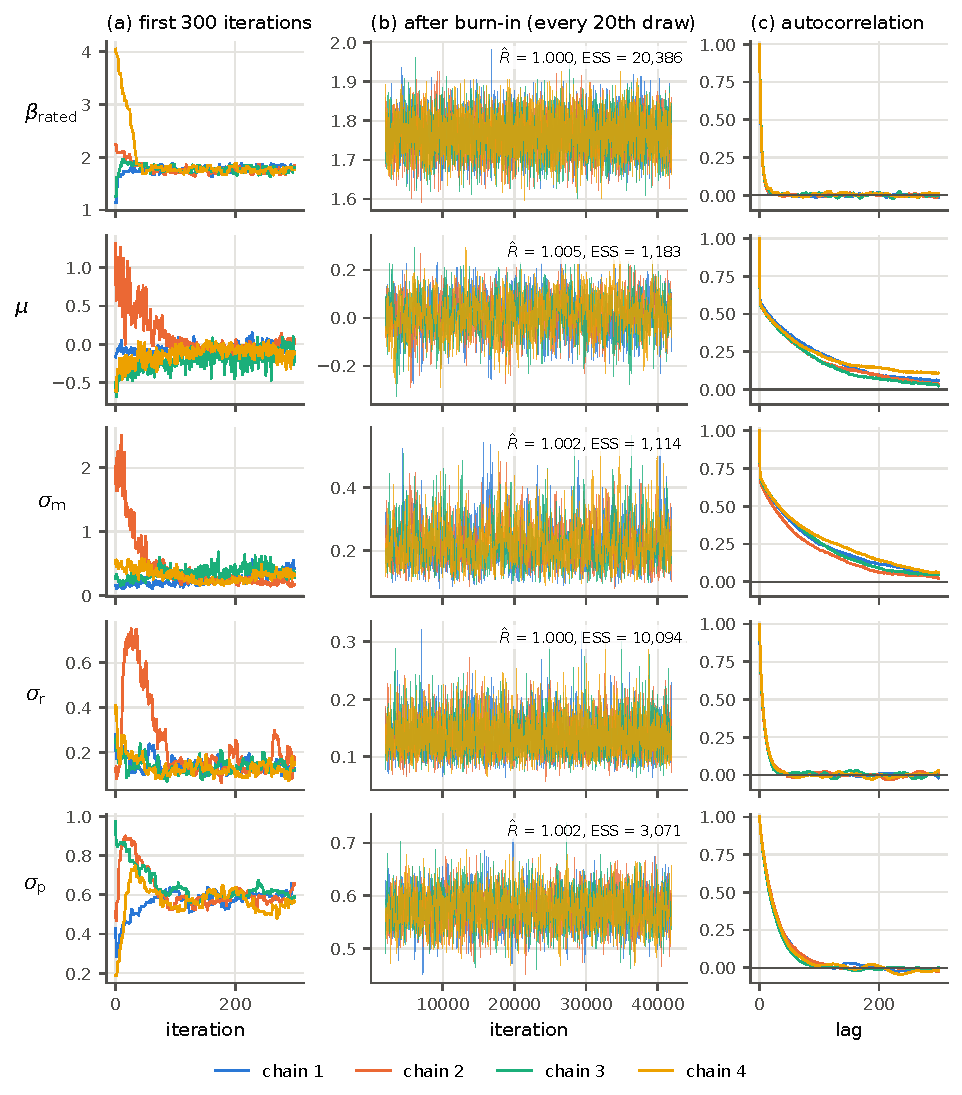
\includegraphics[width=\linewidth]{trace_full.pdf}
  \caption{Convergence of the sampler of the final model on the real data: 4 chains started from points drawn from the prior. (a): the first 300 iterations; (b): the 40,000 iterations kept per chain after a burn-in of 2,000, with the split-$\hat R$ and the effective sample size (ESS) of the four chains together; (c): autocorrelation of each chain after burn-in. The slope $\beta$ mixes fast. The spreads of the replies and of the players, which have moves that rescale their whole level at once, reach an ESS of 10,094 and 3,071; $\mu$ and $\sigma_{\mathrm{m}}$, learned from only 20 first moves, are the slowest, with an ESS of 1,183 and 1,114, still enough for small Monte Carlo errors.}
  \label{fig:trace_full}
\end{figure}


\section{Code}\label{app:code}

{\sloppy The code in \texttt{code/} runs from start to end with \texttt{python run\_all.py}, and its \texttt{README.md} lists which script produces each figure and table. The samplers and diagnostics are our own (\texttt{sampler.py}, \texttt{sampler\_moves.py}, \texttt{sampler\_full.py}, \texttt{diagnostics.py}); NumPy, SciPy \citep{virtanen2020scipy}, pandas and Matplotlib \citep{hunter2007matplotlib} serve for random numbers, linear algebra, data handling and figures. Every number of this report is written into \texttt{report/generated/} by \texttt{make\_report\_numbers.py} from the tables of the analysis.\par}

\end{document}
